\documentclass[11pt,a4paper]{book} % Basisdokumentenklasse

\usepackage{amsmath,amssymb,amsthm}
\usepackage{pgf, tikz}
\usetikzlibrary{decorations.pathreplacing}
\usetikzlibrary{positioning,shapes,shadows,arrows}
\usepackage{xspace}
\usepackage{typearea}
\usepackage{lmodern}
\usepackage{stmaryrd}
\usepackage{fancyhdr}
\usepackage{listings}
\usepackage[T1]{fontenc}
\usepackage[utf8]{inputenc}
\usepackage[ngerman, english]{babel}
\usepackage[inner=3cm,outer=2cm,top=3cm,bottom=2.5cm]{geometry}
\usepackage{textcomp}
\usepackage[hyperfootnotes=false,bookmarksopen=true]{hyperref}
\usepackage{algorithm}
\usepackage{verbatim}
\usepackage{fancyvrb}
\usepackage{algpseudocode}
\usepackage{cite}
\usepackage{enumerate}
\usepackage{multicol}
\usepackage{graphicx}
\usepackage{oldgerm}
\usepackage{subfigure}
\usepackage{setspace}
\usetikzlibrary{arrows,shapes,positioning,automata}
\usepackage{booktabs}
\usepackage{tabularx}
\usepackage{multirow}
\usepackage{todonotes}
\usepackage{wrapfig}

\usepackage{mdframed}
\usepackage[section]{placeins}

\allowdisplaybreaks

%%%%%%%%%%%%%%%%%%%%%%%%%%%%%%%%%%%%%%%%%%%%%%%%%%%%%%%%
\pagestyle{fancyplain}

\lhead[\fancyplain{}{\thepage}]{\fancyplain{}{\let\uppercase\relax\sl\rightmark}}
\chead{}
\rhead[\fancyplain{}{\let\uppercase\relax\sl\leftmark}]{\fancyplain{}{\thepage}}
\cfoot{}
\pagenumbering{arabic}
\makeatletter
\def\cleardoublepage{\clearpage\if@twoside\ifodd\c@page\else
	\hbox{}
	\thispagestyle{empty}
	\newpage
	\if@twocolumn\hbox{}\newpage\fi\fi\fi}
\makeatother

\lstset{
	backgroundcolor=\color{white},	% choose the background color
	basicstyle=\ttfamily,			% the size of the fonts that are used for the code
	breakatwhitespace=false,		% sets if automatic breaks should only happen at whitespace
	breaklines=true,				% sets automatic line breaking
	captionpos=b,					% sets the caption-position to bottom
	commentstyle=\color{green!60!black},% comment style
	deletekeywords={...},			% if you want to delete keywords from the given language
	escapeinside={\%*}{*)},			% if you want to add LaTeX within your code
	frame=none,					% adds a frame around the code
	keepspaces=false,				% keeps spaces in text, useful for keeping indentation of code
	% (possibly needs columns=flexible)
	keywordstyle=\color{blue},		% keyword style
	lineskip=0.1pt,
	%linewidth=0.7\linewidth,
	frame=lines,
	morekeywords={*,...},			% if you want to add more keywords to the set
	numbers=left,				% where to put the line-numbers; possible values are (none, left, right)
	numbersep=5pt,				% how far the line-numbers are from the code
	numberstyle=\tiny\color{gray},		% the style that is used for the line-numbers
	rulecolor=\color{black},			% if not set, the frame-color may change on line-breaks within not-black text
	showspaces=false,				% show spaces using underscores; overrides 'showstringspaces'
	showstringspaces=false,			% underline spaces within strings only
	showtabs=false,				% show tabs within strings adding particular underscores
	stepnumber=1,				% the step between two line-numbers. If it's 1, each line will be numbered
	stringstyle=\color{mymauve},		% string literal style
	tabsize=2,					% sets default tabsize to 2 spaces
	%title=\lstname	,				% show the filename of files included with \lstinputlisting; also try caption instead of title
	xleftmargin=2cm,
	xrightmargin=2cm
} 


%%%%%%%%%%%%%%%%%%%%%%%%%%%%%%%%%%%%%%%%%%%%%%%%%%%%%%%%
\newcommand{\definitionautorefname}{Definition}
\newcommand{\exampleautorefname}{Example}
\newcommand{\listingautorefname}{Figure}

\newcommand{\code}[1]{\textit{#1}}
\newcommand{\tool}[1]{\textsf{#1}}
\newcommand{\aprove}{\tool{AProVE}\xspace}
\newcommand{\HRule}[1]{\rule{\linewidth}{#1}}
\newcommand{\stem}{\textit{STEM}\xspace}
\newcommand{\loopt}{\textit{LOOP}\xspace}
\newcommand{\guardmatrix}{\textit{Guard Matrix}\xspace}
\newcommand{\guardconstants}{\textit{Guard Constants}\xspace}
\newcommand{\updatematrix}{\textit{Update Matrix}\xspace}
\newcommand{\updateconstants}{\textit{Update Constants}\xspace}
\newcommand{\iterationmatrix}{\textit{Iteration Matrix}\xspace}
\newcommand{\iterationconstants}{\textit{Iteration Constants}\xspace}
\newcommand{\startterm}{\textit{start term}\xspace}
\newcommand{\gna}{\textit{geometric nontermination argument}\xspace}
\newcommand{\gnanal}{\textit{geometric nontermination analysis}\xspace}
\newcommand{\rpntree}{\textit{Reverse Polish Notation Tree}\xspace}
\newcommand{\smtfactory}{\code{SMTFactory}}
\newcommand{\its}{\tool{int-TRS}\xspace}
\newcommand{\llvm}{\tool{llvm}\xspace}

\newtheorem{definition}{Definition}[section]
\newtheorem{corollary}{Corollary}[section]
\newtheorem{example}{Example}
\newtheorem{satz}{Satz}[chapter]
\newtheoremstyle{example}{5pt}{5pt}{}{}{\bfseries}{.}{0.5em}{}

\begin{document}

% Einrücken von Absätzen verhindern und 1.5 Zeilen Absatzabstand
\setlength{\parindent}{0pt}
\setlength{\parskip}{1.5ex plus0.5ex minus0.5ex}

%\begin{titlepage}
%	\begin{center}
%		\huge \textbf{\textsf{Geometric Non-Termination Arguments for Integer Programs}} \\
%		\vspace{2cm}
%		\LARGE\textbf{\textsc{Bachelor-Thesis}}\\
%		\vspace{1cm}
%		\normalsize
%		vorgelegt am: \today \\
%		\vspace{2.5cm}
%		\large \textbf{at the Lehr- und Forschungsgebiet Informatik 2}\\
%		\large \textbf{Rheinisch Westfälische Technische Hochschule Aachen}\\
%		\vspace{3cm}
%	\end{center}
%	\normalsize{
%		\begin{tabular}{ll}
%			Name: & {Timo Bergerbusch} \\
%			Matrikelnummer: & {344408} \\
%			Studiengang: & Informatik\\
%			Studienjahrgang: & 2017\\
%			Erstgutachter: & {Jera Hensel} \\
%			Zweitgutachter: & {Prof. Dr. Noll} \\
%		\end{tabular}\\
%	}
%\end{titlepage}

\title{ \normalsize \textsc{Bachelor Thesis}
	\\ [2.0cm]
	\HRule{0.5pt} \\
	\LARGE \textbf{Geometric Non-Termination Arguments for Integer Programs}
	\HRule{2pt} \\ [0.5cm]
	\normalsize \today \vspace*{5\baselineskip}}

\date{}

\author{
	Timo Bergerbusch\\ 
	Rheinisch Westfälisch Technische Hochschule Aachen \\
	Lehr- und Forschungsgebiet Informatik 2  \\ \\
	First Referee: Prof. Dr. Jürgen Giesl \\
	Second Referee: apl. Prof. Dr. Thomas Noll \\
	Supervisor: Jera Hensel
	}

\maketitle % English cover

%\clearpage
{\bf\Large Acknowledgement} \\ [1em] 

First, I would like to thank Prof. Dr. Jürgen Giesl for giving me the opportunity to work on an ongoing and relevant topic.
Secondly, I would like to thank apl. Prof. Dr. Thomas Noll for agreeing to be the second referee of my thesis.

Thirdly, I would like to thank Jera Hensel, who supervised me during my thesis. I want to thank her for the many patient answers she gave my no matter how obvious the solution was. She did not only answer questions, but also got proactive herself and helped me creating better results by pointing out my failures and encouraging me during the whole process. Also I want to thank her for the possibility to write the underlying program the way I wanted to without any restrictions or limits regarding the way of approaching the topic. 

Also I want to thank my girlfriend Nadine Vinkelau and all my friends, who encouraged me during my whole studies and not only accepted that I often was short on time, but also backed me up during the whole process. Especially I want to thank my good friend Tobias Räwer, who explained many topics to me over and over again throughout the whole Bachelor studies to help me pass my exams without demanding anything in return. Thanks to his selfless behaviour I got this far within only three years.

Finally I want to thank my parents for giving me the possibility to fulfil my desire to study at a worldwide known university. Without the financial support I would not have had this opportunity. \\ \\

\paragraph{Erklärung} Ich versichere hiermit, dass ich die vorliegende Arbeit selbstständig verfasst und keine
anderen als die angegebenen Quellen und Hilfsmittel benutzt sowie Zitate kenntlich
gemacht habe.\newline \\
Aachen, den \myformat\today

\begin{tabular}{lp{2em}l} 
	\hspace{4cm} \\\cline{1-1}\cline{3-3} 
	Timo Bergerbusch
\end{tabular}


%\clearpage
\newpage
{\bf\Large Abstract} \\ [1em] 

% motivation
The topic of program termination analysis undergoes a significant importance increase owed to the expansion of software usage throughout everyday life. Since fixing problems caused by software bugs leads to an overhead of support, the initial guarantee of correctness can save time spent on fixing these problems. Therefore the research of automated assisting during the engineering of large programs is a growing field.
% problem statement
One major point of a correct program is determined by its termination, which means that it reaches a final state after finitely many steps. Even though such a tool can never provide soundness and completeness at the same time in every condition since it would have to solve the \textit{halting problem}, which is proven by Turing to be undecidable, a variety of tools addressing this problem exist, for example \aprove. \aprove tries to prove (non-)termination for as many programs possible, although not all programs can be handled.\newline \\
% approach
In this thesis we extend the possibilities of proving \nonterm using \aprove by a special set of programs based on the approach described in \cite{leike2014geometric} by Jan Leike and Matthias Heizmann. Altering the underlying structure from linear loop programs to integer transition systems (ITS) we prove \nonterm using a \textit{\gna} derived from the program itself. By the usage of linear algebra and \solver we are able to prove the existence of a \gna, which results in a proof of \nonterm of the integer transition system. Using this technique as an additional approach in \aprove increases its power to prove \nonterm. 
%We restrict ourselves to only have linear updates of the variables in order to be able to apply the underlying approach, which provides correctness and soundness for this particular set of programs.\newline
\\
% results
As a result we will see that the implemented technique provides a mechanism of proving \nonterm for different programs. For some of them \nonterm could not be proven before. Restricting the set of considered programs to certain criteria defined within this thesis, we are able to prove \nonterm and in special cases we are able to prove termination instead. \newline
 %%%%%%%
\\
% conclusion
In summary we can say that the use of \gnas is a promising approach to prove \nonterm of \itss, as it is for linear lasso programs. The restriction to only use linear updates and its consequences regarding modern programs need further investigation to evaluate the applicability in real industrial software.
 

\tableofcontents

% Ab erstem Kapitel Seiten arabisch zählen
\setcounter{page}{1}
\pagenumbering{arabic}

\chapter{Introduction}

\section{Motivation}
The topic of verification and termination analysis of software increases in importance with the development of new programs. Even though that for Touring Complete programming languages the Halting-Problem is undecidable, and therefore no complete and sound method can exist, a verity of approaches to determine termination are researched and still being developed. These approaches can determine termination on programs, which match certain criteria in form of structure, composition or using only a closed set of operations for example only linear updates of variables. \newline
Given a tool, which can provide a sound and in many scenarios applicable mechanism to prove termination, a optimized framework could analyse written code and find bugs before the actual release of the software \cite{verschaetse1993automatic}. Contemplating that automatic verification can be applied to termination proved software the estimated annual US Economy loses of \$60 billion each year in costs associated software could be reduced significantly \cite{zhivich2009real}. \newline

\section{\emph{AProVE}}
\label{sec:aprove}
One promising approach is the tool \aprove (\underline{A}utomated \underline{Pro}gram \underline{V}erification \underline{E}nvironment) developed at the RWTH Aachen by the Lehr- und Forschungsgebiet Informatik 2. The \emph{AProVE}-tool (further only called \aprove) for automatic termination and complexity proving works with different programming languages of major language paradigms like \tool{Java} (object oriented), \tool{Haskell} (functional), \tool{Prolog} (logical) as well as \tool{rewrite systems}.
\begin{figure}[H]
	\centering
	\begin{tikzpicture}
		\node[aproveNode] at (0,0) (java) {Java};
		\node[aproveNode]at (0,-.75) (c) {C};
		\node[aproveNode] at (0,-1.5) (haskell) {Haskell};
		\node[aproveNode] at (0,-2.25) (prolog) {Prolog};
		\node[shape = circle, draw,align = center] at (3, -1.125) (seg) {Symbolic\\ Execution\\ Tree};
		\node[stdNode] at (6,-.75) (its) {\its};
		\node[stdNode, minimum width = 3cm] at (10,-.25) (comp) {Complexity};
		\node[stdNode, minimum width = 3cm] at (10,-1) (term) {Termination};
		\node[stdNode, minimum width = 3cm] at (10,-1.75) (nterm) {Non-Termination};
		
		\draw[thickarrow] (java) edge (seg);
		\draw[thickarrow] (c) edge (seg);
		\draw[thickarrow] (haskell) edge (seg);
		\draw[thickarrow] (prolog) edge (seg);
		
		\draw[thickarrow] (seg) edge (its);
		\draw[thickarrow] (seg) edge (nterm.west);
		
		\draw[thickarrow] (its) edge (term);
		\draw[thickarrow] (its) edge (comp);
		\draw[thickarrow] (its) edge (nterm);
		
		\draw [thick,decoration={brace,mirror},decorate] (-1,-2.75) -- (3.9,-2.75) 
		node [pos=0.5,anchor=north,yshift=-0.3cm] {\footnotesize Frontends}; 
		
		\draw [thick,decoration={brace,mirror},decorate] (5.2,-2.75) -- (11.5,-2.75) 
		node [pos=0.5,anchor=north,yshift=-0.3cm] {\footnotesize Backend}; 
	\end{tikzpicture}
	\caption{Schematic partition of the derivation process of \aprove adapted from \cite{giesl2017analyzing}}
	\label{fig:aprove-graph}
\end{figure}
\aprove is able to unify different languages into one structure by converting programs of specific languages like \tool{C} into \textit{Low Level Virtual Machine(\llvm)}-code using the tool \tool{Clang} \footnote{further information: \url{https://clang.llvm.org/}}. Among others these \llvm-programs can be converted into a so called \seg. If this graph contains \lasso's, which are strongly connected components (SCC) and the corresponding path from the root to the SCC, \aprove derives so called (integer) term rewrite systems (further only called \its)\footnote{a mathematical definition can be found within \cite{fuhs2009proving}}. By adding conditions to the \its rules the solution space gets restricted and therefore the \its under-approximates. From that it is proven that the non-termination of (at least) one \its implies non-termination of the program. A more detailed description of the process is stated in \cite{hensel2017aprove} \newline
The conversion of different languages into \its and subsequently applying various different approaches is what makes this tool strong in meanings of proofing \cite{giesl2017analyzing}.

\section{Overview}
\label{sec:overview}
This paper provides the introduction to the topic of termination analysis. We focus on the very basic steps, because of the huge variety of possible approaches and related methods. Any further knowledge about termination analysis techniques and how they are applied within \aprove can be found in the related papers \cite{giesl2017analyzing}, \cite{giesl2006aprove}, \cite{giesl2003aprove}.\newline
Within \autoref{chapter:preliminaries} some preliminaries used within the paper are defined to create a well-defined base for any further argumentation and derivation. It covers the topics of basic knowledge about \textit{Integer Term Rewrite Systems} and it's within this approach considered subset based on it's structure. Also the definition of the \gna, which builds the main constituent, and any strongly related matrices are defined. Also we define a tree-structure, which we use to handle arithmetical terms containing variables. Last we take a glimpse at the topic of \tool{SMT}-solving and declare the essential parts used within the implementation of the approach.\newline
The main chapter, which is \autoref{chapter:geo-non-term}, deals with the derivation of the \stem part, for constant or variable terms, the derivation of the \loopt with all it's matrices and finally the derivation of the \tool{SMT}-Problem, which provides a \gna if it exists. \newline
At the end, we want to take a look at the usability of the approach itself. Also we want to point out possible adaptations and improvements of the implementation of this approach.
\chapter{Preliminaries}
\label{chapter:preliminaries}

In order to be able to explain the new \nonterm approach we have to declare, what \nonterm means, which programs are considered within this approach and present the construction of \gnas (GNAs), which builds the core of the approach. Furthermore we have to define a few structures we work on, we have to define what an \solver is and how it is used within this implementation.

%\section{Non-Termination}
%The definition of \nonterm is the most essential considering a technique proving it. Non-termination can be defined as a specific input to a program $p$, such that $p$ runs in an infinite loop.
%Proving termination is much harder than proving \nonterm, since we only have to determine one case, which fit's the condition of running into an infinite loop. \newline
%Non-termination is obviously still undecidable, since otherwise the halting problem would be decidable, nevertheless there are a large variety of possibilities to prove \nonterm as we will see in this paper.

\section{Integer Transition Systems}
\label{sec:its}
In order to apply the upcoming procedure we have to define what structure the approach works on. As described in \Cref{sec:aprove}, the C program is transferred into a symbolic execution graph. Afterwards, from each lasso of the graph an ITS is constructed. Here, a cycle is a lasso together with the path from the initial state to this cycle. Then, if we know that the resulting ITSs has the property that it is equivalent to the original program in its termination behaviour, we can prove non-termination of the original program by proving non-termination of one of the ITSs. Considering the following approach we will look at \itss of a special form shown in \Cref{fig:its-structure}.\newline
\begin{figure}[H]
	\begin{lstlisting}[escapechar=!]
		!$\overbrace{f_x}^{(1)} \qquad\qquad \rightarrow \overbrace{f_y}^{(2)} (v_1, \dots v_n) :|: cond_1$!
		!$\>f_y(\underbrace{v_1, \dots v_n}_{(3)}) \> \rightarrow \>\> f_y \>(\underbrace{v^\prime_1,\dots v^\prime_n}_{(3)})  :|: \underbrace{cond_2}_{(4)}$!
	\end{lstlisting}
	\caption{The structure of an \its considered in this thesis}
	\label{fig:its-structure}
\end{figure}
%QUESTION: Explanation in text or in figure?

The \its shown in \Cref{fig:its-structure} consists of a set of structure elements, whose definition is necessary:
\begin{enumerate}[leftmargin=1]
	\item[(line 1)] The first line is the rewriting rule the program starts with and can be seen as a declaration of initial values of some variables. An example is shown in \Cref{fig:structure-example-TRS}.
	\item[(line 2)] A self-looping rule. Other looping rules will be presented in \Cref{sec:structure-improvement}.
	\item[(1)] The \textit{start function symbol} is the first symbol used, consisting of a function symbol without arguments. Further explanation in (line 1) and \Cref{fig:structure-example-TRS}.
	\item[(2)] A function symbol denoting a current program state
	\item[(3)] The arguments of a function symbol showing the update of the values by applying this rule. The value of $v^\prime_i$ is a linear update of the variables $v_j$, $1 \le j \le n$, in \stdLinInt. \footnote{The \stdLinInt has the following pattern: $ a_1*v_1 + \dots + a_n*v_n + c$, where $a_i , c \in \mathbb{Z}$, $1 \le i\le n$. }
%		Also it is important that $a_i * v_i$ has this order and not $v_i*a_i$} 
	\item[(4)] The conditional term of the form $\text{(in)equation}_1 \text{ \&\& } \dots \text{ \&\& } \text{(in)equation}_m$, $m \in \mathbb{N}$, where $\text{(in)equation}_i$ does not only contain the variables $v_j$, $1 \le j \le n$, but can also introduce new variables. The form of the (in)equalities is defined in \Cref{sec:derivation-guard}.	
\end{enumerate} 

\begin{definition}[run]
	A run of an integer transitioning system is the successively applying of rules, starting from a start function symbol.
\end{definition}

The termination of an \its is now defined as the not existing of an infinite run, i.e. for every run we reach a state in which we can not apply any rule. Vice versa non-termination of an \its is defined as the existence of an infinite run.

%In general an \its can have rules of other forms, like $f_x(v_1, \dots v_n) \rightarrow f_y(v^\prime_1, \dots v^\prime_k) :|: cond$ where $n \ne k$ can occur, but these rules are for now not considered.

\section{geometric non-termination arguments}
Adapted from Jan Leikes and Matthias Heizmanns paper \textit{geometric non-termination arguments (GNA)} \cite{leike2014geometric} we will define the considered programs, define the division of these programs into \stem and \loopt and finally give the definition of \textit{geometric non-termination arguments}.

\subsection{Considered Programs}
The considered programs are not bound to a special programming language. The paper works on so called \textit{linear lasso programs}, which in fact are also used within \aprove. Instead of the linear lasso programs, \aprove represents them as ITSs, stated in \Cref{sec:aprove}. Because of the also stated conversion of the program into a \seg and because of the further analysis the applicability of GNAs is not bound to any programming language. \newline
In order to define the specific conditions under which we can use the approach, we choose the language \tool{Java} as an example.
\subsection{Structure}
\label{sec:structure}
The structure of the considered programs is quite simple. It contains an optional initialization  of the used variables and a \code{while}-loop. Even though \tool{C} would not accept the usage of a variable without declaration, the conversion to \llvm would still be sound. An example of a linear lasso program in \tool{C} is shown in \Cref{fig:structure-example-java}. 
\begin{itemize}
	\item The \stem: \newline
		The declaration and optional initialization of variables used within the \code{while}-loop. In \Cref{fig:structure-example-java} lines 3 and 4 are considered the \stem. Only $b$ is initialized with a value.
	\item The guard: \newline
		The guard of the \code{while}-loop is essential to restrict the variable $a$ as we will see in \Cref{sec:stem-var}. With the restriction of $a+b\ge 4 $ we can prove termination for an initial value of $a < 3$ without further analysis, and also, in order to prove \nonterm, assume that initially $a \ge 3$.
	\item The linear updates: \newline
		The updates of the variables within the \code{while}-loop are the most essential part for termination, since their values determine if the guard still holds. The approach only works with linear updates of the variables, so for every variable $v_i$ where $1\le i\le n$ we can have an update of the form $v_i=a_1*v_1+...+a_n*v_n+c$ with $a_i \in \mathbb{Z}$ for $1 \le i \le n$ and $c \in \mathbb{Z}$.
\end{itemize} 

\begin{figure}[h]
	\begin{lstlisting}[language = java, escapechar = !, linewidth=0.6\linewidth]
	int main(){
		
		int a;!\tikz[remember picture] \node [] (a) {};!
		int b=1;!\tikz[remember picture] \node [] (b) {};!
		
		while(a+b>=4){! \tikz[remember picture] \node [] (c) {}; !
			a=3*a+b;!\tikz[remember picture] \node [] (d) {}; !
			b=2*b-5;!\tikz[remember picture] \node [] (e) {}; !
		}
	}		
	\end{lstlisting}
	\begin{tikzpicture}[remember picture, overlay, 
		every edge/.append style = {dashedarrow},
		every node/.append style = {explNode},
	text width = 2.5cm ]
		\node[above right = .2cm and 3.1 cm of a] (A) {the \textit{STEM}};
		\draw[rounded corners=5pt] (A.west) edge (a.east);
		\draw (A.west) edge (b.east);
		
		\node[below = of A, right = of c] (B) {the guard};
		\draw (B.west) edge (c.east);
		
		\node[right = 4cm of d, below = of B] (C) {the linear update};
		\draw (C.west) edge (d.east);
		\draw (C.west) edge (e.east);
	\end{tikzpicture}
	\caption{A linear lasso program fulfilling the conditions mentioned in \Cref{sec:structure} to be applicable}
	\label{fig:structure-example-java}
\end{figure}
The guard and linear updates together form the so called \loopt. 

%Through the in \Cref{sec:its} described procedure and given structure we receive the to \Cref{fig:structure-example-java} corresponding \its shown in \Cref{fig:structure-example-TRS}. 
The program from \Cref{fig:structure-example-java} can be transformed into the ITS shown in \Cref{fig:structure-example-TRS}, which is conform to the structure described in \Cref{sec:structure}.
As we can see, the original program can be recognized quite easily. The first rule in line 1 represents the \stem, while the second line forms the \loopt. \newline

%TODO: richtig formatieren
\begin{figure}[H]	
	\begin{lstlisting}[linewidth=1.2\textwidth, escapechar = !]
!$\overbrace{f_1	     \rightarrow f_2(1+3*v_1,-3)   :|: v_1>2 \text{ \&\& } 8<3*v_1}^{\text{\stem}}$!
!$f_2(v_1,v_2) \rightarrow f_2(3*v_1+v_2,v_3) :|: v_1 + v_2 > 3 \text{ \&\& } v_1 > 6 \text{ \&\& } 3 * v_1 > 20 \text{ \&\& }$!
!$\underbrace{\text{\qquad\qquad\qquad\qquad\qquad\qquad}}_{\text{linear update}}$!		!$\underbrace{ 5 + v_3 = 2 * v_2 \text{ \&\& } v_3 < -10\text{\qquad\qquad\qquad} }_{\text{guards}}$!
!$\underbrace{\text{\qquad\qquad\qquad\qquad\qquad\qquad\qquad\qquad\qquad\qquad\qquad\qquad\qquad\qquad\qquad\qquad}}_{\text{\loopt}}$!
	\end{lstlisting}

	\caption{The \its corresponding to the \tool{Java} program in \Cref{fig:structure-example-java}}
	\label{fig:structure-example-TRS}
\end{figure}
%TODO: beispiel ändern
 Neglecting the conditional terms for now, the declaration of $v^\prime_2$, which is the second argument of $f_2$, in line 1 to -3, 
 because during the construction of the \seg, \aprove always unrolls the first iteration of the \loopt. Therefore, the \stem computed by \aprove will always contain the first execution of the \loopt. Starting with $b=1$ one step would be the computation of $b = 2*1-5=-3$. The definition of $v^\prime_1$ is more difficult and will be shown within \Cref{sec:stem}.
Also the update for the first argument of $f_2$ $v^\prime_1$ within line 2 is the same as in \Cref{fig:structure-example-java} line 7. The definition of the second argument of $f_2$, $v^\prime_2 = v_3$, is fundamental and not as simple as $v^\prime_1$, since $v_3$ is a new variable introduced within the guards through the equality $5+v_3=2*v_2$. The handling of such variables will be explained in \Cref{sec:derivation-guard} and \Cref{sec:derivation-update}. \newline

\subsection{Preliminary Definitions}
In order to be able to define the key element of this approach, the \gna, we have to define a number of matrices and constant vectors, which are used to derive such a \gna. 

\begin{definition}[\stem]
	The \stem is denoted as a vector $x \in \mathbb{Z}^n$, where $n$ is the number of variables within the rule of the start function symbols right hand side of a \its. The values of $x$ can be constants or defined by conditions. Examples are shown within \Cref{sec:stem}.
\end{definition}

\begin{definition}[Guard Matrix, Guard Constants]
	\label{def:guard}
	Let $n \in \mathbb{N}$ be the number of distinct variables, $v_i$ $1 \le i \le n$ the $i$-th distinct variable names occurring on the left hand side, $m \in \mathbb{N}$ be the number of guards not containing equality, $a_{i,j} \in \mathbb{Z}$ $1\le i \le n$, $1 \le j \le m$ the factor of $v_i$ in $g_j$ and $c_i \in \mathbb{Z}$ be the constant term within $r_j$. \newline
	
	Then the \guardmatrix $G \in \mathbb{Z}^{m\times n}$ is defined as $G_{i,j}=a_{i,j} $ and \guardconstants $g \in \mathbb{Z}^m$ are defined as $g_i = c_i$.
	
	Newly introduced variables must not be represented by a column of the \guardmatrix, but create substitutions further used in \Cref{sec:stem-var}, \Cref{sec:derivation-guard} and \Cref{sec:derivation-update}.
\end{definition}
\begin{example}
	The corresponding \guardmatrix to \Cref{fig:structure-example-TRS} is $G = \begin{pmatrix} -1 & -1 \\ -1 & 0 \\ -3 & 0 \\ 0 & 2 \end{pmatrix}$ and the \guardconstants is $g= \begin{pmatrix} -4 \\ -7 \\ -21 \\ -6 \end{pmatrix}$ \newline
	The normalization of the guards $r_i$ to the form $a_{i,1}v_1+\dots a_{i,n}v_n \le c$ transforms for example the guard $r_1$ in the following way
	\begin{center}
		$r_1 \Leftrightarrow v_1+v_2 > 3  \Leftrightarrow -v_1-v_2 < -3 \Leftrightarrow -v_1-v_2 \le -4$
	\end{center}
\end{example}

\begin{definition}[Update Matrix, Update Constants]
	\label{def:update}
	Let $n \in \mathbb{N}$ be the number of distinct variables of the left hand side, $v_i$ $1 \le i \le n$ the $i$-th distinct		variable name, $m \in \mathbb{N}$ the arity of the function symbol of the right hand side, $v^\prime_i$ $1 \le i \le m$ the $i$-th variable definition of the right hand sight's function symbol, $a_{i,j} \in \mathbb{Z}$ $1 \le i \le n$ $1 \le j \le m$ be the factor of variable $v_i$ in variable definition $v^\prime_i$ and $c_i \in \mathbb{Z}$ $1 \le i \le m$ the constant term of $v^\prime_i$. \newline
	
	Then the \updatematrix $U \in \mathbb{Z}^{m \times n}$ is defined as $U_{i,j}=a_{i,j}$ and \updateconstants $u \in \mathbb{Z}^m$ are defined as $g_i = c_i$.
	
	Regarding the new variable $v_3$, we have to substitute in order to keep the desired size of the matrix. This procedure is further defined within \Cref{sec:derivation-guard} and \Cref{sec:derivation-update}.
\end{definition}
\begin{example}
	The corresponding \updatematrix to \Cref{fig:structure-example-TRS} is $U = \begin{pmatrix} 3 & 1 \\ 0 & 2 \end{pmatrix}$ and the \updateconstants are $u = \begin{pmatrix} 0 \\ -5 \end{pmatrix}$.
	
	The second row is not as obvious as the first row and will be derived in detail within \Cref{sec:derivation-update}.
\end{example}

\begin{definition}[Iteration Matrix, Iteration Constants]
	\label{def:iteration}
	Let $G$ be the \guardmatrix, $g$ the \guardconstants, $U$ the \updatematrix, $u$ the \updateconstants, $n\in \mathbb{N}$ the number of variables and $m \in \mathbb{N}$ the number of conditional terms. \newline
	Also let \textbf{0} be a matrix of the size of $G$ with only entry's 0 and $I$ denote the identity matrix having the same dimension as $U$. \newline
	
	The \iterationmatrix $A \in \mathbb{Z}^{2*n+m \times 2*n}$, which defines one complete execution of the \loopt, and the \iterationconstants $b\in \mathbb{Z}^{2*n+m} $ is defined as
	\begin{figure}[H]
		\centering
		$A = \begin{pmatrix} G & \textbf{0} \\ U & -I \\ -U & I \end{pmatrix}$ and $b = \begin{pmatrix} g \\ -u \\ u \end{pmatrix}$ \cite{leike2014geometric}
	\end{figure}	
\end{definition}

\begin{definition}[LOOP]
	The \loopt is defined as a tuple $(A, b)$, where $A$ is the \iterationmatrix and $b$ the \iterationconstants of an \its.
\end{definition}

Now we can define the key element, which was originally defined for \tool{linear lasso programs}. 

\begin{definition}[geometric non-termination argument]
	\label{def:gna}
	A tuple of the form:
	\begin{figure}[H]
		\centering
		$(x, y_1, \dots, y_k, \lambda_1, \dots, \lambda_k, \mu_1, \dots, \mu_{k-1})$
	\end{figure}  
	\vspace{-1em}
	is called a \gna of size $k$ for a program = $(\stem, \loopt)$ with $n$ variables iff all of the following statements hold:
	\begin{itemize}
		\setlength{\itemindent}{1in}
		\item[(domain)] $x, y_1, \dots, y_k \in \mathbb{R}^n$, $\lambda_1, \dots \lambda_k, \mu_1, \dots \mu_{k-1} \ge 0$
		\item[(init)] x represents the \startterm (\stem)
		\item[(point)] $A\begin{pmatrix} x \\ x + \sum_i y_i \end{pmatrix} \le b$
		\item[(ray)] $A\begin{pmatrix} y_i \\ \lambda_i y_i + \mu_{i-1} y_{i-1} \end{pmatrix} \le 0$ for all $1 \le i \le k$
	\end{itemize}
	Note that $y_0 = \mu_0 = 0$ is set for the ray instead of a case distinction. \cite{leike2014geometric}
\end{definition}

The usage of such a \gna is justified by the following sentence:
\begin{satz}
	\label{sen:gna-nonterm}
	If a \gna $a$ for a program $p$ exists, then $p$ does not terminate. \cite{leike2014geometric} 
\end{satz}

\section{Reverse-Polish-Notation-Tree}
\label{sec:rpntree}
Within the program of deriving a \gna it happens that we get a mathematical term in the so-called \textit{Polish Notation} or \textit{Reverse Polish Notation in prefix notation}, which is a special form of rewriting a, in our case linear, expression to compute the solution efficiently using a stack.\cite{wikirpn} Within our program we use this kind of notation to parse it into our own tree-structure to do further analysis.

As shown in \Cref{dia:RPN-classdiagram} we have an \code{abstract} root, subclasses for every occurring type of element within the \its, a \code{static} parsing of a given term and an exception for parsing exceptions.
An example of the \rpntree's usage is shown in \Cref{ex:rpntree}

\begin{figure}[H]
	\centering
	% Graphic for TeX using PGF
% Title: D:\Dokumente\GitHub\Bachelorarbeit\Arbeitstagebuch\src\04.07.2017-RPNTree-classdiagram.dia
% Creator: Dia v0.97.2
% CreationDate: Wed Aug 30 19:22:10 2017
% For: Timo Bergerbusch
% \usepackage{tikz}
% The following commands are not supported in PSTricks at present
% We define them conditionally, so when they are implemented,
% this pgf file will use them.
\ifx\du\undefined
  \newlength{\du}
\fi
\setlength{\du}{15\unitlength}
\begin{tikzpicture}[scale=0.5, every node/.style={scale=0.5}]
\pgftransformxscale{1.000000}
\pgftransformyscale{-1.000000}
\definecolor{dialinecolor}{rgb}{0.000000, 0.000000, 0.000000}
\pgfsetstrokecolor{dialinecolor}
\definecolor{dialinecolor}{rgb}{1.000000, 1.000000, 1.000000}
\pgfsetfillcolor{dialinecolor}
\pgfsetlinewidth{0.010000\du}
\pgfsetdash{}{0pt}
\definecolor{dialinecolor}{rgb}{1.000000, 1.000000, 1.000000}
\pgfsetfillcolor{dialinecolor}
\fill (-2.412990\du,34.090900\du)--(-2.412990\du,64.000000\du)--(60.422652\du,64.000000\du)--(60.422652\du,34.090900\du)--cycle;
\definecolor{dialinecolor}{rgb}{0.000000, 0.000000, 0.000000}
\pgfsetstrokecolor{dialinecolor}
\draw (-2.412990\du,34.090900\du)--(-2.412990\du,64.000000\du)--(60.422652\du,64.000000\du)--(60.422652\du,34.090900\du)--cycle;
\definecolor{dialinecolor}{rgb}{1.000000, 1.000000, 1.000000}
\pgfsetfillcolor{dialinecolor}
\fill (-2.412990\du,33.090900\du)--(-2.412990\du,34.090900\du)--(7.412010\du,34.090900\du)--(7.412010\du,33.090900\du)--cycle;
\definecolor{dialinecolor}{rgb}{0.000000, 0.000000, 0.000000}
\pgfsetstrokecolor{dialinecolor}
\draw (-2.412990\du,33.090900\du)--(-2.412990\du,34.090900\du)--(7.412010\du,34.090900\du)--(7.412010\du,33.090900\du)--cycle;
% setfont left to latex
\definecolor{dialinecolor}{rgb}{0.000000, 0.000000, 0.000000}
\pgfsetstrokecolor{dialinecolor}
\node[anchor=west] at (-2.312990\du,33.790900\du){ReversePolishNotationTree};
\pgfsetlinewidth{0.010000\du}
\pgfsetdash{}{0pt}
\definecolor{dialinecolor}{rgb}{1.000000, 1.000000, 1.000000}
\pgfsetfillcolor{dialinecolor}
\fill (23.800000\du,34.400000\du)--(23.800000\du,36.600000\du)--(44.705000\du,36.600000\du)--(44.705000\du,34.400000\du)--cycle;
\definecolor{dialinecolor}{rgb}{0.000000, 0.000000, 0.000000}
\pgfsetstrokecolor{dialinecolor}
\draw (23.800000\du,34.400000\du)--(23.800000\du,36.600000\du)--(44.705000\du,36.600000\du)--(44.705000\du,34.400000\du)--cycle;
% setfont left to latex
\definecolor{dialinecolor}{rgb}{0.000000, 0.000000, 0.000000}
\pgfsetstrokecolor{dialinecolor}
\node at (34.252500\du,35.160000\du){<<abstract>>};
% setfont left to latex
\definecolor{dialinecolor}{rgb}{0.000000, 0.000000, 0.000000}
\pgfsetstrokecolor{dialinecolor}
\node at (34.252500\du,36.200000\du){RPNNode};
\definecolor{dialinecolor}{rgb}{1.000000, 1.000000, 1.000000}
\pgfsetfillcolor{dialinecolor}
\fill (23.800000\du,36.600000\du)--(23.800000\du,37.000000\du)--(44.705000\du,37.000000\du)--(44.705000\du,36.600000\du)--cycle;
\definecolor{dialinecolor}{rgb}{0.000000, 0.000000, 0.000000}
\pgfsetstrokecolor{dialinecolor}
\draw (23.800000\du,36.600000\du)--(23.800000\du,37.000000\du)--(44.705000\du,37.000000\du)--(44.705000\du,36.600000\du)--cycle;
\definecolor{dialinecolor}{rgb}{1.000000, 1.000000, 1.000000}
\pgfsetfillcolor{dialinecolor}
\fill (23.800000\du,37.000000\du)--(23.800000\du,49.200000\du)--(44.705000\du,49.200000\du)--(44.705000\du,37.000000\du)--cycle;
\definecolor{dialinecolor}{rgb}{0.000000, 0.000000, 0.000000}
\pgfsetstrokecolor{dialinecolor}
\draw (23.800000\du,37.000000\du)--(23.800000\du,49.200000\du)--(44.705000\du,49.200000\du)--(44.705000\du,37.000000\du)--cycle;
% setfont left to latex
\definecolor{dialinecolor}{rgb}{0.000000, 0.000000, 0.000000}
\pgfsetstrokecolor{dialinecolor}
\node[anchor=west] at (23.950000\du,37.660000\du){+getFactorOfVar(varName:String): int};
% setfont left to latex
\definecolor{dialinecolor}{rgb}{0.000000, 0.000000, 0.000000}
\pgfsetstrokecolor{dialinecolor}
\node[anchor=west] at (23.950000\du,38.460000\du){+getConstantTerm(): int};
% setfont left to latex
\definecolor{dialinecolor}{rgb}{0.000000, 0.000000, 0.000000}
\pgfsetstrokecolor{dialinecolor}
\node[anchor=west] at (23.950000\du,39.260000\du){+containsVar(varName:String): boolean};
% setfont left to latex
\definecolor{dialinecolor}{rgb}{0.000000, 0.000000, 0.000000}
\pgfsetstrokecolor{dialinecolor}
\node[anchor=west] at (23.950000\du,40.060000\du){+containsEquality(): boolean};
% setfont left to latex
\definecolor{dialinecolor}{rgb}{0.000000, 0.000000, 0.000000}
\pgfsetstrokecolor{dialinecolor}
\node[anchor=west] at (23.950000\du,40.860000\du){+normalize(): RPNNode};
% setfont left to latex
\definecolor{dialinecolor}{rgb}{0.000000, 0.000000, 0.000000}
\pgfsetstrokecolor{dialinecolor}
\node[anchor=west] at (23.950000\du,41.660000\du){+remove(rem:RPNNode): RPNNode};
% setfont left to latex
\definecolor{dialinecolor}{rgb}{0.000000, 0.000000, 0.000000}
\pgfsetstrokecolor{dialinecolor}
\node[anchor=west] at (23.950000\du,42.460000\du){+getConstantNode(): RPNConstant};
% setfont left to latex
\definecolor{dialinecolor}{rgb}{0.000000, 0.000000, 0.000000}
\pgfsetstrokecolor{dialinecolor}
\node[anchor=west] at (23.950000\du,43.260000\du){+<<abstract>> negate(): RPNNode};
% setfont left to latex
\definecolor{dialinecolor}{rgb}{0.000000, 0.000000, 0.000000}
\pgfsetstrokecolor{dialinecolor}
\node[anchor=west] at (23.950000\du,44.060000\du){+<<abstract>> clone(): RPNNode};
% setfont left to latex
\definecolor{dialinecolor}{rgb}{0.000000, 0.000000, 0.000000}
\pgfsetstrokecolor{dialinecolor}
\node[anchor=west] at (23.950000\du,44.860000\du){+<<abstract>> applySubstitution(var:RPNVariable,};
\definecolor{dialinecolor}{rgb}{0.000000, 0.000000, 0.000000}
\pgfsetstrokecolor{dialinecolor}
\node[anchor=west] at (23.950000\du,45.660000\du){                                sub:RPNNode): RPNNode};
% setfont left to latex
\definecolor{dialinecolor}{rgb}{0.000000, 0.000000, 0.000000}
\pgfsetstrokecolor{dialinecolor}
\node[anchor=west] at (23.950000\du,46.460000\du){+toString(): String};
% setfont left to latex
\definecolor{dialinecolor}{rgb}{0.000000, 0.000000, 0.000000}
\pgfsetstrokecolor{dialinecolor}
\node[anchor=west] at (23.950000\du,47.260000\du){+toPrefixString(): String};
% setfont left to latex
\definecolor{dialinecolor}{rgb}{0.000000, 0.000000, 0.000000}
\pgfsetstrokecolor{dialinecolor}
\node[anchor=west] at (23.950000\du,48.060000\du){+toInfixString(): String};
% setfont left to latex
\definecolor{dialinecolor}{rgb}{0.000000, 0.000000, 0.000000}
\pgfsetstrokecolor{dialinecolor}
\node[anchor=west] at (23.950000\du,48.860000\du){+toSuffixString(): String};
\pgfsetlinewidth{0.010000\du}
\pgfsetdash{}{0pt}
\definecolor{dialinecolor}{rgb}{1.000000, 1.000000, 1.000000}
\pgfsetfillcolor{dialinecolor}
\fill (38.000000\du,50.000000\du)--(38.000000\du,51.400000\du)--(60.060000\du,51.400000\du)--(60.060000\du,50.000000\du)--cycle;
\definecolor{dialinecolor}{rgb}{0.000000, 0.000000, 0.000000}
\pgfsetstrokecolor{dialinecolor}
\draw (38.000000\du,50.000000\du)--(38.000000\du,51.400000\du)--(60.060000\du,51.400000\du)--(60.060000\du,50.000000\du)--cycle;
% setfont left to latex
\definecolor{dialinecolor}{rgb}{0.000000, 0.000000, 0.000000}
\pgfsetstrokecolor{dialinecolor}
\node at (49.030000\du,51.000000\du){RPNVariable};
\definecolor{dialinecolor}{rgb}{1.000000, 1.000000, 1.000000}
\pgfsetfillcolor{dialinecolor}
\fill (38.000000\du,51.400000\du)--(38.000000\du,52.400000\du)--(60.060000\du,52.400000\du)--(60.060000\du,51.400000\du)--cycle;
\definecolor{dialinecolor}{rgb}{0.000000, 0.000000, 0.000000}
\pgfsetstrokecolor{dialinecolor}
\draw (38.000000\du,51.400000\du)--(38.000000\du,52.400000\du)--(60.060000\du,52.400000\du)--(60.060000\du,51.400000\du)--cycle;
% setfont left to latex
\definecolor{dialinecolor}{rgb}{0.000000, 0.000000, 0.000000}
\pgfsetstrokecolor{dialinecolor}
\node[anchor=west] at (38.150000\du,52.060000\du){-varName: String};
\definecolor{dialinecolor}{rgb}{1.000000, 1.000000, 1.000000}
\pgfsetfillcolor{dialinecolor}
\fill (38.000000\du,52.400000\du)--(38.000000\du,55.800000\du)--(60.060000\du,55.800000\du)--(60.060000\du,52.400000\du)--cycle;
\definecolor{dialinecolor}{rgb}{0.000000, 0.000000, 0.000000}
\pgfsetstrokecolor{dialinecolor}
\draw (38.000000\du,52.400000\du)--(38.000000\du,55.800000\du)--(60.060000\du,55.800000\du)--(60.060000\du,52.400000\du)--cycle;
% setfont left to latex
\definecolor{dialinecolor}{rgb}{0.000000, 0.000000, 0.000000}
\pgfsetstrokecolor{dialinecolor}
\node[anchor=west] at (38.150000\du,53.060000\du){+RPNVariable(varName:String)};
% setfont left to latex
\definecolor{dialinecolor}{rgb}{0.000000, 0.000000, 0.000000}
\pgfsetstrokecolor{dialinecolor}
\node[anchor=west] at (38.150000\du,53.860000\du){+negate(): RPNNode};
% setfont left to latex
\definecolor{dialinecolor}{rgb}{0.000000, 0.000000, 0.000000}
\pgfsetstrokecolor{dialinecolor}
\node[anchor=west] at (38.150000\du,54.660000\du){+clone(): RPNNode};
% setfont left to latex
\definecolor{dialinecolor}{rgb}{0.000000, 0.000000, 0.000000}
\pgfsetstrokecolor{dialinecolor}
\node[anchor=west] at (38.150000\du,55.460000\du){+applySubstitution(var:RPNVariable,sub:RPNNode): RPNNode};
\pgfsetlinewidth{0.010000\du}
\pgfsetdash{}{0pt}
\definecolor{dialinecolor}{rgb}{1.000000, 1.000000, 1.000000}
\pgfsetfillcolor{dialinecolor}
\fill (38.000000\du,57.000000\du)--(38.000000\du,58.400000\du)--(60.060000\du,58.400000\du)--(60.060000\du,57.000000\du)--cycle;
\definecolor{dialinecolor}{rgb}{0.000000, 0.000000, 0.000000}
\pgfsetstrokecolor{dialinecolor}
\draw (38.000000\du,57.000000\du)--(38.000000\du,58.400000\du)--(60.060000\du,58.400000\du)--(60.060000\du,57.000000\du)--cycle;
% setfont left to latex
\definecolor{dialinecolor}{rgb}{0.000000, 0.000000, 0.000000}
\pgfsetstrokecolor{dialinecolor}
\node at (49.030000\du,58.000000\du){RPNConstant};
\definecolor{dialinecolor}{rgb}{1.000000, 1.000000, 1.000000}
\pgfsetfillcolor{dialinecolor}
\fill (38.000000\du,58.400000\du)--(38.000000\du,59.400000\du)--(60.060000\du,59.400000\du)--(60.060000\du,58.400000\du)--cycle;
\definecolor{dialinecolor}{rgb}{0.000000, 0.000000, 0.000000}
\pgfsetstrokecolor{dialinecolor}
\draw (38.000000\du,58.400000\du)--(38.000000\du,59.400000\du)--(60.060000\du,59.400000\du)--(60.060000\du,58.400000\du)--cycle;
% setfont left to latex
\definecolor{dialinecolor}{rgb}{0.000000, 0.000000, 0.000000}
\pgfsetstrokecolor{dialinecolor}
\node[anchor=west] at (38.150000\du,59.060000\du){-value: int};
\definecolor{dialinecolor}{rgb}{1.000000, 1.000000, 1.000000}
\pgfsetfillcolor{dialinecolor}
\fill (38.000000\du,59.400000\du)--(38.000000\du,63.600000\du)--(60.060000\du,63.600000\du)--(60.060000\du,59.400000\du)--cycle;
\definecolor{dialinecolor}{rgb}{0.000000, 0.000000, 0.000000}
\pgfsetstrokecolor{dialinecolor}
\draw (38.000000\du,59.400000\du)--(38.000000\du,63.600000\du)--(60.060000\du,63.600000\du)--(60.060000\du,59.400000\du)--cycle;
% setfont left to latex
\definecolor{dialinecolor}{rgb}{0.000000, 0.000000, 0.000000}
\pgfsetstrokecolor{dialinecolor}
\node[anchor=west] at (38.150000\du,60.060000\du){+RPNConstant(value:int)};
% setfont left to latex
\definecolor{dialinecolor}{rgb}{0.000000, 0.000000, 0.000000}
\pgfsetstrokecolor{dialinecolor}
\node[anchor=west] at (38.150000\du,60.860000\du){+<<override>> getConstantNode(): RPNConstant};
% setfont left to latex
\definecolor{dialinecolor}{rgb}{0.000000, 0.000000, 0.000000}
\pgfsetstrokecolor{dialinecolor}
\node[anchor=west] at (38.150000\du,61.660000\du){+negate(): RPNNode};
% setfont left to latex
\definecolor{dialinecolor}{rgb}{0.000000, 0.000000, 0.000000}
\pgfsetstrokecolor{dialinecolor}
\node[anchor=west] at (38.150000\du,62.460000\du){+clone(): RPNNode};
% setfont left to latex
\definecolor{dialinecolor}{rgb}{0.000000, 0.000000, 0.000000}
\pgfsetstrokecolor{dialinecolor}
\node[anchor=west] at (38.150000\du,63.260000\du){+applySubstitution(var:RPNVariable,sub:RPNNode): RPNNode};
\pgfsetlinewidth{0.010000\du}
\pgfsetdash{}{0pt}
\definecolor{dialinecolor}{rgb}{1.000000, 1.000000, 1.000000}
\pgfsetfillcolor{dialinecolor}
\fill (10.000000\du,54.000000\du)--(10.000000\du,55.400000\du)--(32.060000\du,55.400000\du)--(32.060000\du,54.000000\du)--cycle;
\definecolor{dialinecolor}{rgb}{0.000000, 0.000000, 0.000000}
\pgfsetstrokecolor{dialinecolor}
\draw (10.000000\du,54.000000\du)--(10.000000\du,55.400000\du)--(32.060000\du,55.400000\du)--(32.060000\du,54.000000\du)--cycle;
% setfont left to latex
\definecolor{dialinecolor}{rgb}{0.000000, 0.000000, 0.000000}
\pgfsetstrokecolor{dialinecolor}
\node at (21.030000\du,55.000000\du){RPNFunctionSymbol};
\definecolor{dialinecolor}{rgb}{1.000000, 1.000000, 1.000000}
\pgfsetfillcolor{dialinecolor}
\fill (10.000000\du,55.400000\du)--(10.000000\du,58.000000\du)--(32.060000\du,58.000000\du)--(32.060000\du,55.400000\du)--cycle;
\definecolor{dialinecolor}{rgb}{0.000000, 0.000000, 0.000000}
\pgfsetstrokecolor{dialinecolor}
\draw (10.000000\du,55.400000\du)--(10.000000\du,58.000000\du)--(32.060000\du,58.000000\du)--(32.060000\du,55.400000\du)--cycle;
% setfont left to latex
\definecolor{dialinecolor}{rgb}{0.000000, 0.000000, 0.000000}
\pgfsetstrokecolor{dialinecolor}
\node[anchor=west] at (10.150000\du,56.060000\du){\#left: RPNNode};
% setfont left to latex
\definecolor{dialinecolor}{rgb}{0.000000, 0.000000, 0.000000}
\pgfsetstrokecolor{dialinecolor}
\node[anchor=west] at (10.150000\du,56.860000\du){\#right: RPNNode};
% setfont left to latex
\definecolor{dialinecolor}{rgb}{0.000000, 0.000000, 0.000000}
\pgfsetstrokecolor{dialinecolor}
\node[anchor=west] at (10.150000\du,57.660000\du){-arithemticSymbol: ArithemticSymbol};
\definecolor{dialinecolor}{rgb}{1.000000, 1.000000, 1.000000}
\pgfsetfillcolor{dialinecolor}
\fill (10.000000\du,58.000000\du)--(10.000000\du,63.800000\du)--(32.060000\du,63.800000\du)--(32.060000\du,58.000000\du)--cycle;
\definecolor{dialinecolor}{rgb}{0.000000, 0.000000, 0.000000}
\pgfsetstrokecolor{dialinecolor}
\draw (10.000000\du,58.000000\du)--(10.000000\du,63.800000\du)--(32.060000\du,63.800000\du)--(32.060000\du,58.000000\du)--cycle;
% setfont left to latex
\definecolor{dialinecolor}{rgb}{0.000000, 0.000000, 0.000000}
\pgfsetstrokecolor{dialinecolor}
\node[anchor=west] at (10.150000\du,58.660000\du){+RPNFunctionSymbol(symbol:ArithemticSymbol,};
\definecolor{dialinecolor}{rgb}{0.000000, 0.000000, 0.000000}
\pgfsetstrokecolor{dialinecolor}
\node[anchor=west] at (10.150000\du,59.460000\du){                   left:RPNNode,right:RPNNode)};
% setfont left to latex
\definecolor{dialinecolor}{rgb}{0.000000, 0.000000, 0.000000}
\pgfsetstrokecolor{dialinecolor}
\node[anchor=west] at (10.150000\du,60.260000\du){+<<override>> remove(rem:RPNNode): RPNNode};
% setfont left to latex
\definecolor{dialinecolor}{rgb}{0.000000, 0.000000, 0.000000}
\pgfsetstrokecolor{dialinecolor}
\node[anchor=west] at (10.150000\du,61.060000\du){+<<override>> getConstantNode(): RPNConstant};
% setfont left to latex
\definecolor{dialinecolor}{rgb}{0.000000, 0.000000, 0.000000}
\pgfsetstrokecolor{dialinecolor}
\node[anchor=west] at (10.150000\du,61.860000\du){+negate(): RPNNode};
% setfont left to latex
\definecolor{dialinecolor}{rgb}{0.000000, 0.000000, 0.000000}
\pgfsetstrokecolor{dialinecolor}
\node[anchor=west] at (10.150000\du,62.660000\du){+clone(): RPNNode};
% setfont left to latex
\definecolor{dialinecolor}{rgb}{0.000000, 0.000000, 0.000000}
\pgfsetstrokecolor{dialinecolor}
\node[anchor=west] at (10.150000\du,63.460000\du){+applySubstitution(var:RPNVariable,sub:RPNNode): RPNNode};
\pgfsetlinewidth{0.010000\du}
\pgfsetdash{}{0pt}
\pgfsetmiterjoin
\pgfsetbuttcap
{
\definecolor{dialinecolor}{rgb}{0.000000, 0.000000, 0.000000}
\pgfsetfillcolor{dialinecolor}
% was here!!!
\definecolor{dialinecolor}{rgb}{0.000000, 0.000000, 0.000000}
\pgfsetstrokecolor{dialinecolor}
\draw (34.252500\du,49.200000\du)--(34.252500\du,51.900000\du)--(38.000000\du,51.900000\du);
}
\definecolor{dialinecolor}{rgb}{0.000000, 0.000000, 0.000000}
\pgfsetstrokecolor{dialinecolor}
\draw (34.252500\du,50.111803\du)--(34.252500\du,51.900000\du)--(38.000000\du,51.900000\du);
\pgfsetmiterjoin
\definecolor{dialinecolor}{rgb}{1.000000, 1.000000, 1.000000}
\pgfsetfillcolor{dialinecolor}
\fill (34.652500\du,50.111803\du)--(34.252500\du,49.311803\du)--(33.852500\du,50.111803\du)--cycle;
\pgfsetlinewidth{0.010000\du}
\pgfsetdash{}{0pt}
\pgfsetmiterjoin
\definecolor{dialinecolor}{rgb}{0.000000, 0.000000, 0.000000}
\pgfsetstrokecolor{dialinecolor}
\draw (34.652500\du,50.111803\du)--(34.252500\du,49.311803\du)--(33.852500\du,50.111803\du)--cycle;
% setfont left to latex
\pgfsetlinewidth{0.010000\du}
\pgfsetdash{}{0pt}
\pgfsetmiterjoin
\pgfsetbuttcap
{
\definecolor{dialinecolor}{rgb}{0.000000, 0.000000, 0.000000}
\pgfsetfillcolor{dialinecolor}
% was here!!!
\definecolor{dialinecolor}{rgb}{0.000000, 0.000000, 0.000000}
\pgfsetstrokecolor{dialinecolor}
\draw (34.252500\du,49.200000\du)--(34.252500\du,60.700000\du)--(38.000000\du,60.700000\du);
}
\definecolor{dialinecolor}{rgb}{0.000000, 0.000000, 0.000000}
\pgfsetstrokecolor{dialinecolor}
\draw (34.252500\du,50.111803\du)--(34.252500\du,60.700000\du)--(38.000000\du,60.700000\du);
\pgfsetmiterjoin
\definecolor{dialinecolor}{rgb}{1.000000, 1.000000, 1.000000}
\pgfsetfillcolor{dialinecolor}
\fill (34.652500\du,50.111803\du)--(34.252500\du,49.311803\du)--(33.852500\du,50.111803\du)--cycle;
\pgfsetlinewidth{0.010000\du}
\pgfsetdash{}{0pt}
\pgfsetmiterjoin
\definecolor{dialinecolor}{rgb}{0.000000, 0.000000, 0.000000}
\pgfsetstrokecolor{dialinecolor}
\draw (34.652500\du,50.111803\du)--(34.252500\du,49.311803\du)--(33.852500\du,50.111803\du)--cycle;
% setfont left to latex
\pgfsetlinewidth{0.010000\du}
\pgfsetdash{}{0pt}
\pgfsetmiterjoin
\pgfsetbuttcap
{
\definecolor{dialinecolor}{rgb}{0.000000, 0.000000, 0.000000}
\pgfsetfillcolor{dialinecolor}
% was here!!!
\definecolor{dialinecolor}{rgb}{0.000000, 0.000000, 0.000000}
\pgfsetstrokecolor{dialinecolor}
\draw (34.252500\du,49.200000\du)--(34.252500\du,54.700000\du)--(32.060000\du,54.700000\du);
}
\definecolor{dialinecolor}{rgb}{0.000000, 0.000000, 0.000000}
\pgfsetstrokecolor{dialinecolor}
\draw (34.252500\du,50.111803\du)--(34.252500\du,54.700000\du)--(32.060000\du,54.700000\du);
\pgfsetmiterjoin
\definecolor{dialinecolor}{rgb}{1.000000, 1.000000, 1.000000}
\pgfsetfillcolor{dialinecolor}
\fill (34.652500\du,50.111803\du)--(34.252500\du,49.311803\du)--(33.852500\du,50.111803\du)--cycle;
\pgfsetlinewidth{0.010000\du}
\pgfsetdash{}{0pt}
\pgfsetmiterjoin
\definecolor{dialinecolor}{rgb}{0.000000, 0.000000, 0.000000}
\pgfsetstrokecolor{dialinecolor}
\draw (34.652500\du,50.111803\du)--(34.252500\du,49.311803\du)--(33.852500\du,50.111803\du)--cycle;
% setfont left to latex
\pgfsetlinewidth{0.010000\du}
\pgfsetdash{}{0pt}
\definecolor{dialinecolor}{rgb}{1.000000, 1.000000, 1.000000}
\pgfsetfillcolor{dialinecolor}
\fill (0.369629\du,44.098102\du)--(0.369629\du,46.298102\du)--(12.5\du,46.298102\du)--(12.5\du,44.098102\du)--cycle;
\definecolor{dialinecolor}{rgb}{0.000000, 0.000000, 0.000000}
\pgfsetstrokecolor{dialinecolor}
\draw (0.369629\du,44.098102\du)--(0.369629\du,46.298102\du)--(12.5\du,46.298102\du)--(12.5\du,44.098102\du)--cycle;
% setfont left to latex
\definecolor{dialinecolor}{rgb}{0.000000, 0.000000, 0.000000}
\pgfsetstrokecolor{dialinecolor}
\node at (6.5\du,44.858102\du){<<enum>>};
% setfont left to latex
\definecolor{dialinecolor}{rgb}{0.000000, 0.000000, 0.000000}
\pgfsetstrokecolor{dialinecolor}
\node at (6.5\du,45.898102\du){ArithmeticSymbol};
\definecolor{dialinecolor}{rgb}{1.000000, 1.000000, 1.000000}
\pgfsetfillcolor{dialinecolor}
\fill (0.369629\du,46.298102\du)--(0.369629\du,52.098102\du)--(12.5\du,52.098102\du)--(12.5\du,46.298102\du)--cycle;
\definecolor{dialinecolor}{rgb}{0.000000, 0.000000, 0.000000}
\pgfsetstrokecolor{dialinecolor}
\draw (0.369629\du,46.298102\du)--(0.369629\du,52.098102\du)--(12.5\du,52.098102\du)--(12.5\du,46.298102\du)--cycle;
% setfont left to latex
\definecolor{dialinecolor}{rgb}{0.000000, 0.000000, 0.000000}
\pgfsetstrokecolor{dialinecolor}
\node[anchor=west] at (0.519629\du,46.958102\du){ PLUS};
% setfont left to latex
\definecolor{dialinecolor}{rgb}{0.000000, 0.000000, 0.000000}
\pgfsetstrokecolor{dialinecolor}
\node[anchor=west] at (0.519629\du,47.758102\du){ MINUS};
% setfont left to latex
\definecolor{dialinecolor}{rgb}{0.000000, 0.000000, 0.000000}
\pgfsetstrokecolor{dialinecolor}
\node[anchor=west] at (0.519629\du,48.558102\du){ TIMES};
% setfont left to latex
\definecolor{dialinecolor}{rgb}{0.000000, 0.000000, 0.000000}
\pgfsetstrokecolor{dialinecolor}
\node[anchor=west] at (0.519629\du,49.358102\du){ LESS\_THAN};
% setfont left to latex
\definecolor{dialinecolor}{rgb}{0.000000, 0.000000, 0.000000}
\pgfsetstrokecolor{dialinecolor}
\node[anchor=west] at (0.519629\du,50.158102\du){ LESS\_THAN\_OR\_EQUAL};
% setfont left to latex
\definecolor{dialinecolor}{rgb}{0.000000, 0.000000, 0.000000}
\pgfsetstrokecolor{dialinecolor}
\node[anchor=west] at (0.519629\du,50.958102\du){ GREATER\_THAN};
% setfont left to latex
\definecolor{dialinecolor}{rgb}{0.000000, 0.000000, 0.000000}
\pgfsetstrokecolor{dialinecolor}
\node[anchor=west] at (0.519629\du,51.758102\du){ GREATER\_THAN\_OR\_EQUAL};
\definecolor{dialinecolor}{rgb}{1.000000, 1.000000, 1.000000}
\pgfsetfillcolor{dialinecolor}
\fill (0.369629\du,52.098102\du)--(0.369629\du,53.098102\du)--(12.5\du,53.098102\du)--(12.5\du,52.098102\du)--cycle;
\definecolor{dialinecolor}{rgb}{0.000000, 0.000000, 0.000000}
\pgfsetstrokecolor{dialinecolor}
\draw (0.369629\du,52.098102\du)--(0.369629\du,53.098102\du)--(12.5\du,53.098102\du)--(12.5\du,52.098102\du)--cycle;
% setfont left to latex
\definecolor{dialinecolor}{rgb}{0.000000, 0.000000, 0.000000}
\pgfsetstrokecolor{dialinecolor}
\node[anchor=west] at (0.519629\du,52.758102\du){+toString(): String};
\pgfsetlinewidth{0.010000\du}
\pgfsetdash{{0.400000\du}{0.400000\du}}{0\du}
\pgfsetdash{{0.200000\du}{0.200000\du}}{0\du}
\pgfsetmiterjoin
\pgfsetbuttcap
{
\definecolor{dialinecolor}{rgb}{0.000000, 0.000000, 0.000000}
\pgfsetfillcolor{dialinecolor}
% was here!!!
\definecolor{dialinecolor}{rgb}{0.000000, 0.000000, 0.000000}
\pgfsetstrokecolor{dialinecolor}
\draw (10.000000\du,56.700000\du)--(6.5\du,56.700000\du)--(6.5\du,53.098102\du);
}
\definecolor{dialinecolor}{rgb}{0.000000, 0.000000, 0.000000}
\pgfsetstrokecolor{dialinecolor}
\draw (9.088197\du,56.700000\du)--(6.5\du,56.700000\du)--(6.5\du,53.098102\du);
\pgfsetmiterjoin
\definecolor{dialinecolor}{rgb}{1.000000, 1.000000, 1.000000}
\pgfsetfillcolor{dialinecolor}
\fill (9.088197\du,57.100000\du)--(9.888197\du,56.700000\du)--(9.088197\du,56.300000\du)--cycle;
\pgfsetlinewidth{0.010000\du}
\pgfsetdash{}{0pt}
\pgfsetmiterjoin
\definecolor{dialinecolor}{rgb}{0.000000, 0.000000, 0.000000}
\pgfsetstrokecolor{dialinecolor}
\draw (9.088197\du,57.100000\du)--(9.888197\du,56.700000\du)--(9.088197\du,56.300000\du)--cycle;
% setfont left to latex
\pgfsetlinewidth{0.010000\du}
\pgfsetdash{}{0pt}
\definecolor{dialinecolor}{rgb}{1.000000, 1.000000, 1.000000}
\pgfsetfillcolor{dialinecolor}
\fill (-1.600000\du,34.800000\du)--(-1.600000\du,36.200000\du)--(18.920000\du,36.200000\du)--(18.920000\du,34.800000\du)--cycle;
\definecolor{dialinecolor}{rgb}{0.000000, 0.000000, 0.000000}
\pgfsetstrokecolor{dialinecolor}
\draw (-1.600000\du,34.800000\du)--(-1.600000\du,36.200000\du)--(18.920000\du,36.200000\du)--(18.920000\du,34.800000\du)--cycle;
% setfont left to latex
\definecolor{dialinecolor}{rgb}{0.000000, 0.000000, 0.000000}
\pgfsetstrokecolor{dialinecolor}
\node at (8.660000\du,35.800000\du){RPNTreeParser};
\definecolor{dialinecolor}{rgb}{1.000000, 1.000000, 1.000000}
\pgfsetfillcolor{dialinecolor}
\fill (-1.600000\du,36.200000\du)--(-1.600000\du,36.600000\du)--(18.920000\du,36.600000\du)--(18.920000\du,36.200000\du)--cycle;
\definecolor{dialinecolor}{rgb}{0.000000, 0.000000, 0.000000}
\pgfsetstrokecolor{dialinecolor}
\draw (-1.600000\du,36.200000\du)--(-1.600000\du,36.600000\du)--(18.920000\du,36.600000\du)--(18.920000\du,36.200000\du)--cycle;
\definecolor{dialinecolor}{rgb}{1.000000, 1.000000, 1.000000}
\pgfsetfillcolor{dialinecolor}
\fill (-1.600000\du,36.600000\du)--(-1.600000\du,37.600000\du)--(18.920000\du,37.600000\du)--(18.920000\du,36.600000\du)--cycle;
\definecolor{dialinecolor}{rgb}{0.000000, 0.000000, 0.000000}
\pgfsetstrokecolor{dialinecolor}
\draw (-1.600000\du,36.600000\du)--(-1.600000\du,37.600000\du)--(18.920000\du,37.600000\du)--(18.920000\du,36.600000\du)--cycle;
% setfont left to latex
\definecolor{dialinecolor}{rgb}{0.000000, 0.000000, 0.000000}
\pgfsetstrokecolor{dialinecolor}
\node[anchor=west] at (-1.450000\du,37.260000\du){+<<static>> parseSetToTree(trsTerm:TRSTerm): RPNNode};
\pgfsetlinewidth{0.010000\du}
\pgfsetdash{}{0pt}
\definecolor{dialinecolor}{rgb}{1.000000, 1.000000, 1.000000}
\pgfsetfillcolor{dialinecolor}
\fill (-1.992776\du,40.200000\du)--(-1.992776\du,41.600000\du)--(19.297224\du,41.600000\du)--(19.297224\du,40.200000\du)--cycle;
\definecolor{dialinecolor}{rgb}{0.000000, 0.000000, 0.000000}
\pgfsetstrokecolor{dialinecolor}
\draw (-1.992776\du,40.200000\du)--(-1.992776\du,41.600000\du)--(19.297224\du,41.600000\du)--(19.297224\du,40.200000\du)--cycle;
% setfont left to latex
\definecolor{dialinecolor}{rgb}{0.000000, 0.000000, 0.000000}
\pgfsetstrokecolor{dialinecolor}
\node at (8.652224\du,41.200000\du){UnsupportedArithmeticSymbolException};
\definecolor{dialinecolor}{rgb}{1.000000, 1.000000, 1.000000}
\pgfsetfillcolor{dialinecolor}
\fill (-1.992776\du,41.600000\du)--(-1.992776\du,42.600000\du)--(19.297224\du,42.600000\du)--(19.297224\du,41.600000\du)--cycle;
\definecolor{dialinecolor}{rgb}{0.000000, 0.000000, 0.000000}
\pgfsetstrokecolor{dialinecolor}
\draw (-1.992776\du,41.600000\du)--(-1.992776\du,42.600000\du)--(19.297224\du,42.600000\du)--(19.297224\du,41.600000\du)--cycle;
% setfont left to latex
\definecolor{dialinecolor}{rgb}{0.000000, 0.000000, 0.000000}
\pgfsetstrokecolor{dialinecolor}
\node[anchor=west] at (-1.842776\du,42.260000\du){-serialVersionUID: static final long};
\definecolor{dialinecolor}{rgb}{1.000000, 1.000000, 1.000000}
\pgfsetfillcolor{dialinecolor}
\fill (-1.992776\du,42.600000\du)--(-1.992776\du,43.600000\du)--(19.297224\du,43.600000\du)--(19.297224\du,42.600000\du)--cycle;
\definecolor{dialinecolor}{rgb}{0.000000, 0.000000, 0.000000}
\pgfsetstrokecolor{dialinecolor}
\draw (-1.992776\du,42.600000\du)--(-1.992776\du,43.600000\du)--(19.297224\du,43.600000\du)--(19.297224\du,42.600000\du)--cycle;
% setfont left to latex
\definecolor{dialinecolor}{rgb}{0.000000, 0.000000, 0.000000}
\pgfsetstrokecolor{dialinecolor}
\node[anchor=west] at (-1.842776\du,43.260000\du){+UnsupportetArithmeticSymbolException(messsage:String)};
\pgfsetlinewidth{0.010000\du}
\pgfsetdash{{0.200000\du}{0.200000\du}}{0\du}
\pgfsetdash{{0.200000\du}{0.200000\du}}{0\du}
\pgfsetmiterjoin
\pgfsetbuttcap
{
\definecolor{dialinecolor}{rgb}{0.000000, 0.000000, 0.000000}
\pgfsetfillcolor{dialinecolor}
% was here!!!
\definecolor{dialinecolor}{rgb}{0.000000, 0.000000, 0.000000}
\pgfsetstrokecolor{dialinecolor}
\draw (18.920000\du,35.500000\du)--(19.770000\du,35.500000\du)--(23.750000\du,35.500000\du)--(23.800000\du,35.500000\du);
}
\definecolor{dialinecolor}{rgb}{0.000000, 0.000000, 0.000000}
\pgfsetstrokecolor{dialinecolor}
\draw (19.831803\du,35.500000\du)--(19.770000\du,35.500000\du)--(23.750000\du,35.500000\du)--(23.800000\du,35.500000\du);
\pgfsetmiterjoin
\definecolor{dialinecolor}{rgb}{1.000000, 1.000000, 1.000000}
\pgfsetfillcolor{dialinecolor}
\fill (19.831803\du,35.100000\du)--(19.031803\du,35.500000\du)--(19.831803\du,35.900000\du)--cycle;
\pgfsetlinewidth{0.010000\du}
\pgfsetdash{}{0pt}
\pgfsetmiterjoin
\definecolor{dialinecolor}{rgb}{0.000000, 0.000000, 0.000000}
\pgfsetstrokecolor{dialinecolor}
\draw (19.831803\du,35.100000\du)--(19.031803\du,35.500000\du)--(19.831803\du,35.900000\du)--cycle;
% setfont left to latex
\pgfsetlinewidth{0.010000\du}
\pgfsetdash{{0.200000\du}{0.200000\du}}{0\du}
\pgfsetdash{{0.200000\du}{0.200000\du}}{0\du}
\pgfsetmiterjoin
\pgfsetbuttcap
{
\definecolor{dialinecolor}{rgb}{0.000000, 0.000000, 0.000000}
\pgfsetfillcolor{dialinecolor}
% was here!!!
\definecolor{dialinecolor}{rgb}{0.000000, 0.000000, 0.000000}
\pgfsetstrokecolor{dialinecolor}
\draw (21.030000\du,54.000000\du)--(21.030000\du,47.100000\du)--(23.800000\du,47.100000\du);
}
\definecolor{dialinecolor}{rgb}{0.000000, 0.000000, 0.000000}
\pgfsetstrokecolor{dialinecolor}
\draw (21.030000\du,53.088197\du)--(21.030000\du,47.100000\du)--(23.800000\du,47.100000\du);
\pgfsetmiterjoin
\definecolor{dialinecolor}{rgb}{1.000000, 1.000000, 1.000000}
\pgfsetfillcolor{dialinecolor}
\fill (20.630000\du,53.088197\du)--(21.030000\du,53.888197\du)--(21.430000\du,53.088197\du)--cycle;
\pgfsetlinewidth{0.010000\du}
\pgfsetdash{}{0pt}
\pgfsetmiterjoin
\definecolor{dialinecolor}{rgb}{0.000000, 0.000000, 0.000000}
\pgfsetstrokecolor{dialinecolor}
\draw (20.630000\du,53.088197\du)--(21.030000\du,53.888197\du)--(21.430000\du,53.088197\du)--cycle;
% setfont left to latex
\pgfsetlinewidth{0.010000\du}
\pgfsetdash{}{0pt}
\pgfsetdash{{0.200000\du}{0.200000\du}}{0\du}
\pgfsetbuttcap
{
\definecolor{dialinecolor}{rgb}{0.000000, 0.000000, 0.000000}
\pgfsetfillcolor{dialinecolor}
% was here!!!
\pgfsetarrowsend{to}
\definecolor{dialinecolor}{rgb}{0.000000, 0.000000, 0.000000}
\pgfsetstrokecolor{dialinecolor}
\draw (8.660000\du,37.600000\du)--(8.652224\du,40.200000\du);
}
% setfont left to latex
\definecolor{dialinecolor}{rgb}{0.000000, 0.000000, 0.000000}
\pgfsetstrokecolor{dialinecolor}
\node[anchor=west] at (8.656107\du,38.699950\du){\{throws\}};
\end{tikzpicture}

%	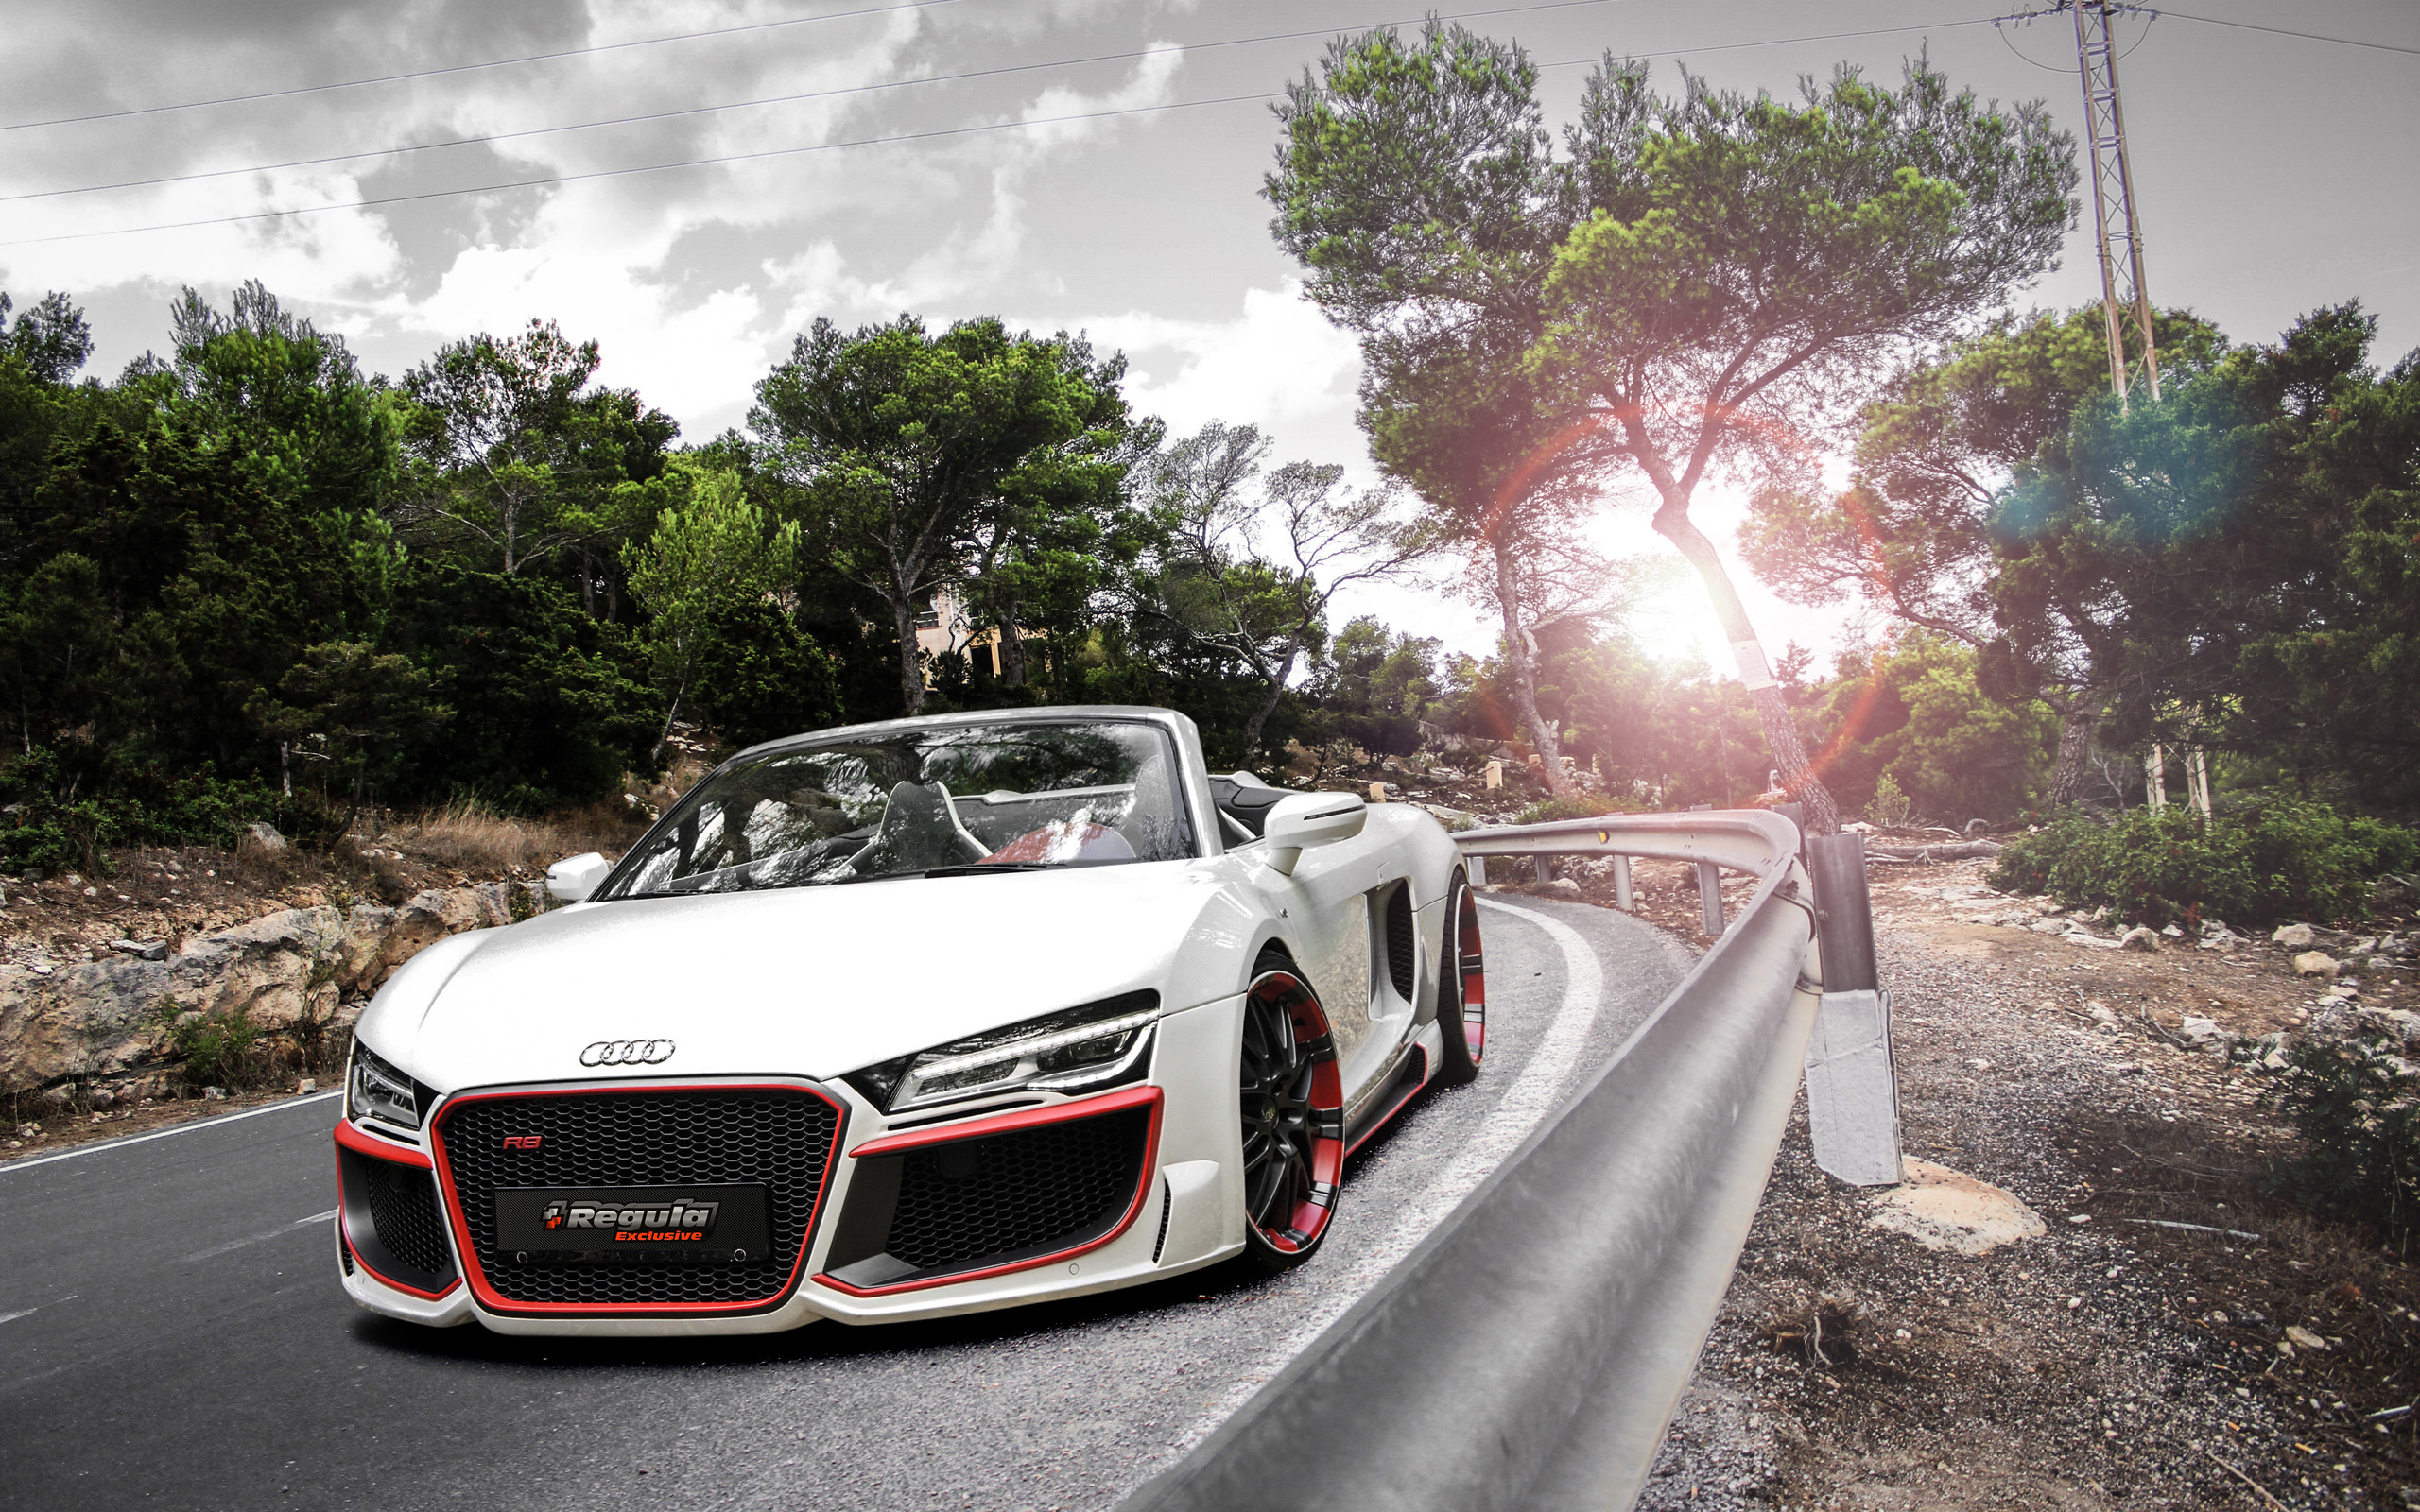
\includegraphics[scale=0.5]{src/diagram/test}
	\caption{The class diagram of the \rpntree within the \gnanal}	
	\label{dia:RPN-classdiagram}
\end{figure}

\newsavebox\mybox
\begin{lrbox}{\mybox}
	\begin{tikzpicture}[scale=0.6, every node/.style={scale=0.6}]
		\node (Plus) at (0,0) [objDia] {
			\textbf{f1}:RPNFunctionSymbol
			\nodepart{second}arithmeticSymbol: PLUS
		};
		\node (Times1) at (-4, -2 ) [objDia] {
			\textbf{f2}:RPNFunctionSymbol
			\nodepart{second}arithmeticSymbol: TIMES	
		};
		\node (cons1) at (-6, -4) [objDia] {
			\textbf{c1}:RPNConstant
			\nodepart{second}value: 3
		};
		\node (var1) at (-2, -4)[objDia] {
			\textbf{v1}:RPNVariable
			\nodepart{second}varName: $v_1$
		};
		\node (var2) at (4, -2) [objDia] {
			\textbf{v2}:RPNVariable
			\nodepart{second}value: $v_2$
		};
		\draw[thickarrow] (Plus.south)  -- ++(0,-0.4) -| (Times1.north) node [pos = 0.4, above, font=\footnotesize]{left};
		\draw[thickarrow] (Plus.south)  -- ++(0,-0.4) -| (var2.north) node [pos = 0.4, above, font=\footnotesize]{right};
		\draw[thickarrow] (Times1.south)  -- ++(0,-0.5) -| (cons1.north) node [pos = 0.4, above, font=\footnotesize]{left};
		\draw[thickarrow] (Times1.south)  -- ++(0,-0.5) -| (var1.north) node [pos = 0.4, above, font=\footnotesize]{right};
	\end{tikzpicture}
\end{lrbox}

\begin{figure}[H]
	\centering
	\begin{tikzpicture}[
			scale=0.6,
			every edge/.append style = { dashedarrow },
			every node/.append style = { stdNode} ]
		\node (L) {\begin{tabular}{cc} mathematical expression: \\ $3*v_1+v_2$ \end{tabular} };
		\node[below = of L] (M)  {\begin{tabular}{cc} reverse polish notation: \\ $+(*(3, v_1),v_2)$ \end{tabular} };
		\node[right = of M] (R) {\usebox\mybox};
		\draw (L.south) edge (M.north);
		\draw (M.east) edge (R.west);
	\end{tikzpicture}
	\caption{An example of the representation of the term $3*v_1+v_2$ as a graph using the \rpntree of \Cref{sec:rpntree}}
	\label{ex:rpntree}
\end{figure}


\section{\tool{SMT}-Problem}
\label{sec:smt-problem}
Also we have to consider an \textit{Satisfiability Modulo Theory}-Problem (\tool{SMT}-Problem), we have to solve to derive a \gna fulfilling all the criterias of \Cref{def:gna}. Since \tool{SMT}-Problem solving is a big research topic on it's own we only consider the very basic of \tool{SMT}-Solving necessary to understand how the program solves the problem. \newline
%TODO: write it more mathematically
Within this approach we use the so called \code{Basic Structures} defined within \aprove to add assertions to the \solver using the \smtfactory. An example of the structure of the assertions can be found in \Cref{ex:assertion-structure}. %MAYBE: Class-dia?

\begin{figure}[H]
	\begin{lstlisting}[escapechar = !]
		!$\underbrace{
			\underbrace{
				\underbrace{\underbrace{3}_{(1)}*\underbrace{v_1}_{(2)}}_{(3)} \quad \underbrace{+}_{(4)} \quad ...
			}_{(5)} 
			\qquad
			\underbrace{\le}_{(6)}
			\qquad
			\underbrace{5}_{(7)}
		}_{(8)}$!
	\end{lstlisting}
	\caption{An example to show the structure of an assertion used for the \solver}
	\label{ex:assertion-structure}
\end{figure}

Such an example assertion can be split into different parts: 
\begin{enumerate}
	\item[(1)] \code{PlainIntegerConstants} as coefficients
	\item[(2)] \code{PlainIntegerVariables'} as variables the \solver should derive values for such that all assertions are satisfied
	\item[(3)] A coefficient multiplied with a variables is represented by an \code{PlainIntegerOperation} with \code{ArithmeticOperationType} \code{MUL} to denote multiplication
	\item[(4)] An \code{ArithmeticOperationType} of type \code{ADD} to denote addition
	\item[(5)] The left hand side is one big \code{PlainIntegerOperation} consisting of the addition(4) of the multiplication (3) of coefficient's (1) and variables (2).
	\item[(6)] The \code{IntegerRelationType} defining the assertion. We only use the \textit{EQ (equal)} or \textit{LE (less than or equal)} relations.
	\item[(7)] The right hand side is only \underline{one} \code{PlainIntegerConstant}
	\item[(8)] The whole line is a \code{PlainIntegerRelation}, which can be transformed into the \code{SMTExpressionFormat} the \solver uses.
\end{enumerate}

We use a solver within \aprove to create a bunch of assertions restricting the possible solution space. Since we operate in integer arithmetic and use linear equations we can restrict the solver to only use \textit{quantifier free linear integer arithmetic}. In order to solve the problem given by the assertions the solver tries to derive a model satisfying all of them or derive an unsatisfiable core. \cite{sat2016}\newline

\begin{example}
	Consider the following assertions that should hold:\newline
	\vspace{-1em}
	\begin{figure}[H]
		\centering
		\begin{tabular}{cccc}
			$x \le y$ &	$x > 5 $ &	$ x+ y \le 20$ &$y \neq 10$ \\
		\end{tabular}
	\end{figure}
	\vspace{-1em}
	Then a possible model would be $m_1 = \{x=6, y=6\}$. An other model would be $m_2 = \{x=6, y=7\}$.
	However If we change the third rule to $x+y\le 10$ there is no model to the problem and we would receive the unsatisfiable core $c= \{x \le y$, $x > 5$, $x+ y \le 10 \}$.
\end{example}

Since for \Cref{def:gna} the existence of a model is the crucial information, the model which should be derived is arbitrary among the set of possible models.

Further knowledge about \tool{SMT}-Problem solving can be gathered from the lecture "Introduction to Satisfiability Checking" or the \tool{SMT-RAT} toolbox for Strategic and Parallel SMT Solving by Prof. Dr. Erika Ábrahám and her team at the \textit{RWTH Aachen University} \cite{corzilius2015smt}.

\chapter{Geometric Non-Termination}

\section{Derivation of the \emph{STEM}}

\section{Derivation of the \emph{LOOP}}

\subsection{The Update Matrix}

\subsection{The Guard Matrix}

\subsection{The Iteration Matrix}

\section{Derivation of the \emph{SMT}-Problem}

\subsection{The Domain Criteria}

\subsection{The Initiation Criteria}

\subsection{The Point Criteria}

\subsection{The Ray Criteria}

\section{Verification of the Geometric Non-Termination Argument}
	 

\chapter{Evaluation and Benchmark}
\label{chapter:eval}
In this chapter we want to take a look at the implementation and evaluate, if the approach itself is useful in terms of applicable cases or if the approach works only on very exotic and uncommon preconditions. \newline
Also we want to take a look at the benchmarks of the implementation, in terms of storage and computational efficiency. \newline
Further we want to outline improvement possibilities of the implementation and problems within, where an efficient solution is not quite obvious.

\section{Evaluation of the approach}
The approach provides a sound and complete solution to specific type of programs. Given a tool like \aprove, which provides an \its the further computation that has to be done can be solved quite efficient. Using an state of the art \solver and the definition of $\lambda_i$ to be the $i$-th eigenvalue the problem can also be resolved efficiently for given $\mu$'s. If the $\mu$'s are not given the problem is undecidable, which makes it still useful within \aprove, but not as strong as before. \newline
Since the paper itself does not mention equalities within the guards the substitution of newly introduced variables as handled within \Cref{sec:derivation-guard} is necessary in order to apply the definition. Such a substitution is very costly in computation time and also highly error prone.

\section{Benchmarks}


STEHT NOCH AUS


\section{Possible Improvement of the Implementation}
The implementation of the approach is fully functional under the circumstances mentioned, like for example the defined structure in \Cref{sec:structure}. Nevertheless also this implementation has certain cases in, which it does not perform as efficient as it could, or where it can be improved in terms of applicability.
So here we state the possible improvements of the implementation to make it universally more useful and therefore stronger or more efficient.
\subsection{\solver logic}
As already stated in \Cref{sec:derivation-smt} the problematic of the $\mu$'s can lead to a shift into undecidability, since the solvating of variable multiplication on integers (\qfnia) is undecidable. Also mentioned in \Cref{sec:derivation-smt} there are a bunch of approaches, which lead to semi-decidability and therefore to the possibility to still use the variable multiplication within the problem if the $\mu$'s can be restricted to a finite domain.\newline
A possible improvement could be an iteration over different values of the $\mu$'s. The number of problems, that have to be solved would be blow up, but the problem itself would always be decidable.\newline
A reliable case-study of a large set of examples could underline the necessity of the iteration, since we wouldn't be able to derive a \gna using the \qfnia. It could also lead to the overhead of computational cost using the iterative method, which can be useful if the problem does not have any time restrictions of the deciding process, but is not suitable within the competitions \aprove participates, like the \textit{International Competition of Termination Tools} \footnote{ further information: \url{http://termination-portal.org/wiki/Termination_Competition} } or \textit{International Competition on Software Verification} \footnote{further information: \url{https://sv-comp.sosy-lab.org/2017/}}. \cite{aproveWebsite} \newline
The \textit{Termination Competition 2017}, which is organized by the \textit{International Competition of Termination Tools}, for example has a time limit of 300 seconds and only allows 4 core usage, which makes an iterative method very costly. \cite{wiki2017termComp}

\subsection{\its program structure}
\label{sec:structure-improvement}
As stated in \Cref{sec:structure} we restrict this implementation to the form 
\begin{figure}[H]
	\begin{lstlisting}[escapechar=!]
	!$f_x \qquad\qquad \>\> \rightarrow f_y (v_1, \dots v_n) \> :|: cond_1$!
	!$f_y(v_1, \dots v_n) \> \rightarrow  f_y \>(v^\prime_1,\dots v^\prime_n)  :|: cond_2$!
	\end{lstlisting}
\end{figure}
which obviously is a restriction, because \its's of the form
\begin{figure}[H]
	\begin{lstlisting}[escapechar=!]
	!$f_x \qquad\qquad \>\ \rightarrow f_y (v_1, \dots v_n) \>\>\> :|: cond_1$!
	!$f_{y_1}(v_1, \dots v_n) \> \rightarrow  f_{y_2} \>(v^\prime_1,\dots v^\prime_n)  :|: cond_2$!
			!$\vdots$!
	!$f_{y_k}(v_1, \dots v_n) \> \rightarrow  f_{y_1} \>(v^\prime_1,\dots v^\prime_n)  :|: cond_{k+1}$!
	\end{lstlisting}
\end{figure}
could possibly considered using the method $k$ times. Analysing such \its would make the implementation much stronger in terms of proofing.
\\
An other possible variation of the considered \its could be like the following
\begin{figure}[H]
	\begin{lstlisting}[escapechar=!]
	!$f_x \qquad\qquad \>\>\>\> \rightarrow f_y (v_1, \dots v_n) \>\> :|: cond_1$!
	!$f_{y_1}(v_1, \dots v_n) \> \rightarrow  f_{y_2} (v^\prime_1,\dots v^\prime_m)  :|: cond_2$!
	!$f_{y_2}(v_1, \dots v_m)  \rightarrow  f_{y_1} (v^\prime_1,\dots v^\prime_n) \> :|: cond_3$!
	\end{lstlisting}
\end{figure}
where $m \ne n$, but the values $v^\prime_i$ $1 \le i \le m$ is computed as a linear update of the values $v_j$ $1 \le j \le n$.

These are only two alternations of the considered structure, which would be also recommended to implement in order to create a more universal applicable method.

\subsection{\rpntree}
Within \Cref{sec:rpntree} we defined the \rpntree, on which we base the arithmetic computations and statements. \aprove also has a tree structure it handles such statements in. The \rpntree structure exists mainly because of two reasons:
\begin{enumerate}
	\item the structure \aprove bases these statements on is much more complex, but also much more powerful, which made programming a lot more difficult. Parsing it into a tree, which can only contain elements expected to be in such expressions not only works equivalently it also prevents errors if \aprove's structure gets extended or changed. The \code{RPNTreeParse} handles the conversion and therefore can be seen as an adapter, which filters every \its that must not occur in \textit{Geometric Nontermination Analysis} as stated in this thesis.
	\item many algorithms are difficult to encode if not programmed recursively. Since coding in the already stated classes was no option, and inheritance would not work because of accessing problems, creating my own structure was a simple work-around.
\end{enumerate}
The examples worked with have been small enough to not create any problems with the conversion and possible less efficient methods, but if applied to huge problems a converting of the approach to work on the structure \aprove proposes would be the better way.
\chapter{related work}



\bibliographystyle{alpha}
\addcontentsline{toc}{chapter}{Literaturverzeichnis}
\bibliography{src/bib/Literatur}

% Begin Anhang
\appendix
%\input{src/tex/appendix_docu}

\end{document}
